% !TeX TS-program = pdflatex


\documentclass[a4paper]{article}

% \usepackage[default]{fontsetup}

\usepackage{fancyhdr}
\usepackage{extramarks}
\usepackage{amsmath}
\usepackage{amsthm}
\usepackage{amsfonts}
\usepackage{tikz}
\usepackage[plain]{algorithm}
\usepackage{algpseudocode}
\usepackage{enumerate}
\usepackage{tikz}

\usetikzlibrary{automata,positioning}

%
% Basic Document Settings
%  

\topmargin=-0.2in
\evensidemargin=0in
\oddsidemargin=0in
\textwidth=6.5in
\textheight=9.5in
\headsep=0.25in

\linespread{1.1}

\pagestyle{fancy}
\lhead{\hmwkAuthorName}
\chead{\hmwkClass : \hmwkTitle}
\rhead{\firstxmark}
\lfoot{\lastxmark}
\cfoot{\thepage}

\renewcommand\headrulewidth{0.4pt}
\renewcommand\footrulewidth{0.4pt}

\setlength\parindent{0pt}

%
% Create Problem Sections
%

\newcommand{\enterProblemHeader}[1]{
    \nobreak\extramarks{}{Problem \arabic{#1} continued on next page\ldots}\nobreak{}
    \nobreak\extramarks{Problem \arabic{#1} (continued)}{Problem \arabic{#1} continued on next page\ldots}\nobreak{}
}

\newcommand{\exitProblemHeader}[1]{
    \nobreak\extramarks{Problem \arabic{#1} (continued)}{Problem \arabic{#1} continued on next page\ldots}\nobreak{}
    \stepcounter{#1}
    \nobreak\extramarks{Problem \arabic{#1}}{}\nobreak{}
}

\newcommand*\circled[1]{\tikz[baseline=(char.base)]{
		\node[shape=circle,draw,inner sep=2pt] (char) {#1};}}


\setcounter{secnumdepth}{0}
\newcounter{partCounter}
\newcounter{homeworkProblemCounter}
\setcounter{homeworkProblemCounter}{1}
\nobreak\extramarks{Problem \arabic{homeworkProblemCounter}}{}\nobreak{}

%
% Homework Problem Environment
%
% This environment takes an optional argument. When given, it will adjust the
% problem counter. This is useful for when the problems given for your
% assignment aren't sequential. See the last 3 problems of this template for an
% example.
%

\newenvironment{homeworkProblem}[1][-1]{
    \ifnum#1>0
        \setcounter{homeworkProblemCounter}{#1}
    \fi
    \section{Problem \arabic{homeworkProblemCounter}}
    \setcounter{partCounter}{1}
    \enterProblemHeader{homeworkProblemCounter}
}{
    \exitProblemHeader{homeworkProblemCounter}
}

%
% Homework Details
%   - Title
%   - Class
%   - Due date
%   - Name
%   - Student ID

\newcommand{\hmwkTitle}{Homework\ \#13}
\newcommand{\hmwkClass}{Probability \& Statistics for EECS}
\newcommand{\hmwkDueDate}{2025-01-07}
\newcommand{\hmwkAuthorName}{Wenye Xiong}
\newcommand{\hmwkAuthorID}{2023533141}


%
% Title Page
%

\title{
    \vspace{2in}
    \textmd{\textbf{\hmwkClass:\\  \hmwkTitle}}\\
    \normalsize\vspace{0.1in}\small{Due\ on\ \hmwkDueDate\ at 11:59}\\
	\vspace{4in}
}

\author{
	Name: \textbf{\hmwkAuthorName} \\
	Student ID: \hmwkAuthorID}
\date{}

\renewcommand{\part}[1]{\textbf{\large Part \Alph{partCounter}}\stepcounter{partCounter}\\}

%
% Various Helper Commands
%

% Useful for algorithms
\newcommand{\alg}[1]{\textsc{\bfseries \footnotesize #1}}
% For derivatives
\newcommand{\deriv}[1]{\frac{\mathrm{d}}{\mathrm{d}x} (#1)}
% For partial derivatives
\newcommand{\pderiv}[2]{\frac{\partial}{\partial #1} (#2)}
% Integral dx
\newcommand{\dx}{\mathrm{d}x}
% Alias for the Solution section header
\newcommand{\solution}{\textbf{\large Solution}}
% Probability commands: Expectation, Variance, Covariance, Bias
\newcommand{\E}{\mathrm{E}}
\newcommand{\Var}{\mathrm{Var}}
\newcommand{\Cov}{\mathrm{Cov}}
\newcommand{\Bias}{\mathrm{Bias}}

\begin{document}


% \maketitle
% \thispagestyle{empty}
% \pagebreak

\date{
Due on Jan. 7, 2025, 11:59 UTC+8}
\title{SI 140A-02  Probability \& Statistics for EECS, Fall 2024 \\
Homework 13}
\maketitle
Read all the instructions below carefully before you start working on the assignment, and before you make a submission.
\begin{itemize}
    \item You are required to write down all the major steps towards making your conclusions; otherwise you may obtain limited points of the problem.
    \item Write your homework in English; otherwise you will get no points of this homework.
    \item Any form of plagiarism will lead to $0$ point of this homework. 
\end{itemize}
\newpage

\begin{homeworkProblem}[1]
Given a Markov chain with state-transition diagram shown as follows:
\begin{center}
    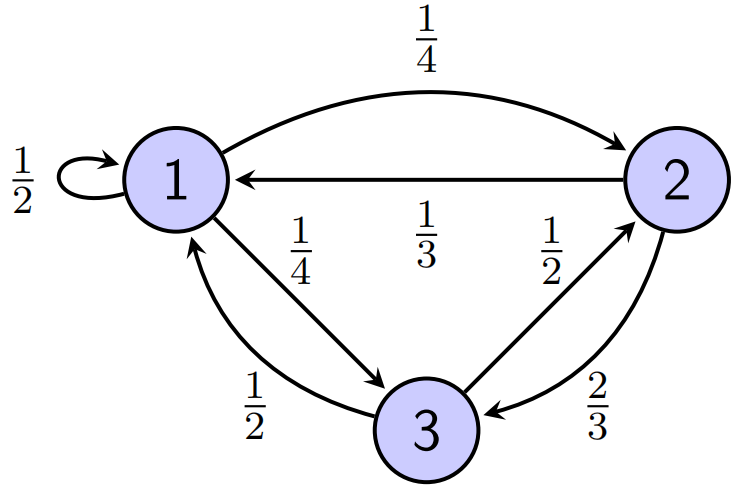
\includegraphics[width=0.3\textwidth]{hw13_1.png}
\end{center}
(a)
Is this chain irreducible?\\[2px]
(b)
Is this chain aperiodic?\\[2px]
(c)
Find the stationary distribution of this chain.\\[2px]
(d)
Is this chain reversible?
\subsection{Solution}
For the Markov chain, we have the transition matrix
    $$
    P=\left[\begin{array}{ccc}
    \frac{1}{2} & \frac{1}{4} & \frac{1}{4} \\
    \frac{1}{3} & 0 & \frac{2}{3} \\
    \frac{1}{2} & \frac{1}{2} & 0
    \end{array}\right]
    $$
\begin{enumerate}[(a)]
    \item Yes, this chain is irreducible because all the elements apart from the diagonal elements are non-zero.
    \item Yes, we can see that 1 is a possible return time for state 1, thus $d(1) = 1$. Since both 2,3 are possible for state 2,3 $d(2) = d(3) = 1$. And because the chain is irreducible, so the chain is aperiodic.
    \item Denote the stationary distribution as $\pi = (\pi_1, \pi_2, \pi_3)$, we have
    \begin{align*}
        \pi P &= \pi\\
        \begin{bmatrix}
            \pi_1 & \pi_2 & \pi_3
        \end{bmatrix}
        \begin{bmatrix}
            \frac{1}{2} & \frac{1}{4} & \frac{1}{4} \\
            \frac{1}{3} & 0 & \frac{2}{3} \\
            \frac{1}{2} & \frac{1}{2} & 0
        \end{bmatrix}
        &=
        \begin{bmatrix}
            \pi_1 & \pi_2 & \pi_3
        \end{bmatrix}
    \end{align*}
    We have the following equations:
    \begin{align*}
        \frac{1}{2}\pi_1 + \frac{1}{3}\pi_2 + \frac{1}{2}\pi_3 &= \pi_1\\
        \frac{1}{4}\pi_1 + \frac{2}{3}\pi_2 + \frac{1}{2}\pi_3 &= \pi_2\\
        \frac{1}{4}\pi_1 + \frac{2}{3}\pi_2 &= \pi_3
    \end{align*}
    Solving the above equations, we have
    \begin{align*}
        \pi_1 &= \frac{16}{35}\\
        \pi_2 &= \frac{9}{35}\\
        \pi_3 &= \frac{2}{7}
    \end{align*}
    Thus, the stationary distribution of this chain is $\pi = \left(\frac{16}{35}, \frac{9}{35}, \frac{2}{7}\right)$.
    \item No, this chain is not reversible. If the chain is reversible, we should have
    \begin{align*}
        \pi_i p_{ij} &= \pi_j p_{ji}
    \end{align*}
    However, we can see that
    \begin{align*}
        \pi_1 p_{12} &= \frac{16}{35} \cdot \frac{1}{4} = \frac{4}{35}\\
        \pi_2 p_{21} &= \frac{9}{35} \cdot \frac{1}{3} = \frac{3}{35}
    \end{align*}
    Thus, the chain is not reversible.

\end{enumerate}
\end{homeworkProblem}

\newpage
\begin{homeworkProblem}[2]
Given a Markov chain with state-transition diagram shown as follows:
\begin{center}
    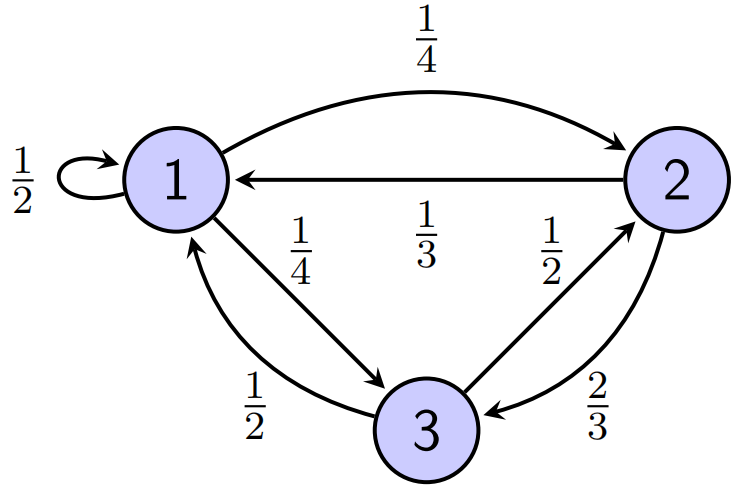
\includegraphics[width=0.3\textwidth]{hw13_1.png}
\end{center}
(a) Find \(P(X_{9}=3 \mid X_{8}=1)\) and \(P(X_{8}=2 \mid X_{7}=3)\).\\[2px]
(b) If \(P(X_{0}=3) = \frac{1}{2}\), find \(P(X_{0}=3, X_{1}=1, X_{2}=2, X_{4}=3)\).\\[2px]
(c) Find \(E(X_{8} \mid X_{6}=2)\).\\[2px]
(d) Find \(\operatorname{Var}(X_{7} \mid X_{5}=3)\).\\[2px]
\subsection{Solution}
For the Markov chain, we have the transition matrix
    $$
    P=\left[\begin{array}{ccc}
    \frac{1}{2} & \frac{1}{4} & \frac{1}{4} \\
    \frac{1}{3} & 0 & \frac{2}{3} \\
    \frac{1}{2} & \frac{1}{2} & 0
    \end{array}\right]
    $$
\begin{enumerate}[(a)]
    \item 
    \begin{align*}
        P(X_{9}=3 \mid X_{8}=1) &= p_{13} = \frac{1}{4}\\
        P(X_{8}=2 \mid X_{7}=3) &= p_{32} = \frac{1}{2}
    \end{align*}
    \item 
    \begin{align*}
        P(X_{0}=3, X_{1}=1, X_{2}=2, X_{4}=3) &= P(X_{0}=3)P(X_{1}=1 \mid X_{0}=3)P(X_{2}=2 \mid X_{1}=1)P(X_{4}=3 \mid X_{2}=2)\\
        &= \frac{1}{2} \cdot \frac{1}{2} \cdot \frac{1}{4} \cdot \frac{1}{12} = \frac{1}{192}
    \end{align*}
    \item 
    $$
    P^2=\left[\begin{array}{ccc}
    \frac{1}{2} & \frac{1}{4} & \frac{1}{4} \\
    \frac{1}{3} & 0 & \frac{2}{3} \\
    \frac{1}{2} & \frac{1}{2} & 0
    \end{array}\right]\left[\begin{array}{ccc}
    \frac{1}{2} & \frac{1}{4} & \frac{1}{4} \\
    \frac{1}{3} & 0 & \frac{2}{3} \\
    \frac{1}{2} & \frac{1}{2} & 0
    \end{array}\right]=\left[\begin{array}{ccc}
    \frac{11}{24} & \frac{1}{4} & \frac{7}{24} \\
    \frac{1}{2} & \frac{5}{12} & \frac{1}{12} \\
    \frac{5}{12} & \frac{1}{8} & \frac{11}{24}
    \end{array}\right]
    $$\\

    $$
    E(X_{8} \mid X_{6}=2) = \sum_{i=1}^{3} i \cdot p_{2i} = 1 \cdot \frac{1}{2} + 2 \cdot \frac{5}{12} + 3 \cdot \frac{1}{12} = \frac{19}{12}
    $$
    
    \item To find \(\operatorname{Var}(X_{7} \mid X_{5}=3)\), we first need to find \(P(X_{7} \mid X_{5}=3)\). We have
    $$
    \operatorname{Var}(X_{7} \mid X_{5}=3) = E(X_{7}^2 \mid X_{5}=3) - E(X_{7} \mid X_{5}=3)^2
    $$
    We have
    $$
    E(X_{7}^2 \mid X_{5}=3) = \sum_{i=1}^{3} i^2 \cdot p_{3i} = 1^2 \cdot \frac{5}{12} + 2^2 \cdot \frac{1}{8} + 3^2 \cdot \frac{11}{24} = \frac{121}{24}
    $$
    $$
    E(X_{7} \mid X_{5}=3) = \sum_{i=1}^{3} i \cdot p_{3i} = 1 \cdot \frac{5}{12} + 2 \cdot \frac{1}{8} + 3 \cdot \frac{11}{24} = \frac{49}{24}
    $$
    Thus, we have
    $$
    \operatorname{Var}(X_{7} \mid X_{5}=3) = \frac{121}{24} - (\frac{49}{24})^2 = \frac{503}{576}
    $$
\end{enumerate}

\end{homeworkProblem}



\newpage
\begin{homeworkProblem}[3]
There are two urns with a total of \(2N\) distinguishable balls. Initially, the first urn has \(N\) white balls and the second urn has \(N\) black balls. At each stage, we pick a ball at random from each urn and interchange them. Let \(X_{n}\) be the number of black balls in the first urn at time \(n\). This is a Markov chain on the state space \(\{0,1,\ldots,N\}\).\\[4px]
(a) Find the transition probabilities of the chain.\\[2px]
(b) Find the stationary distribution of the chain.\\[2px]

\subsection{Solution}
\begin{enumerate}[(a)]
    \item Denote the transition probability as \(p_{ij}\) from i to j. The number of black balls change by at most 1 at each stage. Thus, we have $p_{ij} = 0$ if $|i-j| > 1$.\\
    Also, we have
    $$
        p_{i,i+1} = (\frac{N-i}{N})^2
    $$
    $$
        p_{i,i-1} = (\frac{i}{N})^2
    $$
    And for the number of black balls to stay the same, we have
    $$
        p_{ii} = 1 - p_{i,i+1} - p_{i,i-1} = 1 - \frac{N-i}{N}^2 - \frac{i}{N}^2 = \frac{2i(N-i)}{N^2}
    $$
    \item Denote the stationary distribution as $s = (s_0, s_1, \ldots, s_N)$. 
    According to the result of (a), we have $p_{i,i+1}$ and $p_{i+1,i}$ for each i,
    $$
    p_{i,i+1} = (\frac{N-i}{N})^2
    p_{i+1,i} = (\frac{i+1}{N})^2
    $$
    $$
    p_{i,i-1} = (\frac{i}{N})^2
    p_{i-1,i} = (\frac{N-i+1}{N})^2
    $$
    We have an intuitive guess that the chain is reversible. Thus, to make it, we have
    $$
    s_i p_{i,i+1} = s_{i+1} p_{i+1,i}
    $$
    $$
    s_i p_{i,i-1} = s_{i-1} p_{i-1,i}
    $$
    From that, we made a guess that the stationary distribution should be
    $$
    s_i = \frac{\binom{N}{i} \binom{N}{N-i}}{\binom{2N}{N}}
    $$
    To prove it, we need to show that
    $$
    s_i p_{i,j} = s_j p_{j,i}
    $$ for all i, j.\\
    However, if $|i-j| > 1$, we have $s_i p_{i,j} = 0 = s_j p_{j,i}$. If $i == j$, then both sides are equal to $s_i p_{i,i}$. Thus, we only need to discuss the case where $|i-j| = 1$.\\
    If $j = i+1$, we have
    $$
    s_i p_{i,i+1} = \frac{\binom{N}{i} \binom{N}{N-i}}{\binom{2N}{N}} \cdot (\frac{N-i}{N})^2 = \frac{\binom{N}{i}^2 (N-i)^2}{\binom{2N}{N} N^2}
    $$ and
    $$
    s_{i+1} p_{i+1,i} = \frac{\binom{N}{i+1} \binom{N}{N-i-1}}{\binom{2N}{N}} \cdot (\frac{i+1}{N})^2 = \frac{\binom{N}{i+1}^2 (i+1)^2}{\binom{2N}{N} N^2}
    $$
    We can see that the two sides are equal because
    $$
    \binom{N}{i} (N-i) = \binom{N}{i+1} (i+1)
    $$
    Similarly, we can prove that the two sides are equal when $j = i-1$. 
    $$
    s_i p_{i,i-1} = \frac{\binom{N}{i} \binom{N}{N-i}}{\binom{2N}{N}} \cdot (\frac{i}{N})^2 = \frac{\binom{N}{i}^2 i^2}{\binom{2N}{N} N^2}
    $$ and
    $$
    s_{i-1} p_{i-1,i} = \frac{\binom{N}{i-1} \binom{N}{N-i+1}}{\binom{2N}{N}} \cdot (\frac{N-i+1}{N})^2 = \frac{\binom{N}{i-1}^2 (N-i+1)^2}{\binom{2N}{N} N^2}
    $$
    We can see that the two sides are equal because
    $$
    \binom{N}{i} i = \binom{N}{i-1} (N-i+1)
    $$
    Thus, the stationary distribution of the chain is
    $$
    s_i = \frac{\binom{N}{i} \binom{N}{N-i}}{\binom{2N}{N}}
    $$


\end{enumerate}

\end{homeworkProblem}


\end{document}
